\documentclass[12pt, a4]{article}

% This is the preamble, load any packages you're going to use here
\usepackage{physics} % provides lots of nice features and commands often used in physics, it also loads some other packages (like AMSmath)
\usepackage{siunitx} % typesets numbers with units very nicely
\usepackage{enumerate} % allows us to customize our lists
\usepackage[portuguese]{babel}
\usepackage{float} 
\usepackage{tabto}
\usepackage{graphicx}

\begin{document}

\title{BALANÇO DE ENERGIA EM UM TUBO DE VENTURI}
\author{Luiz Augusto Dembicki Fernandes}
\date{\today}

\maketitle

\begin{abstract}
Foram feitas curvas de energia potencial e cínetica para um tubo de venturi com ar.
O resultado se encontrou parcialmente dentro do esperado.
\end{abstract}

\section{Montagem Experimental}

\tab  Foi utilizado um compressor para encaminhar ar até um tubo de venturi, 
conectado a 8 manometros utilizando água, de forma a medir as pressões(em duas vazões diferentes)
e relacionar com a energia cinética e potencial do ar que trafega o tubo.

\section{Dados}
$ P_{atm} = 692 \ \si{\mmHg} $ \\
$ T_{ambiente} =  23,1 \si{\celsius} $ \\
$ T_{ar} =  31,5 \si{\celsius} $ \\
$ \rho_{ar@31,5 \si{\celsius}} \approx 1.159 \frac{\si{kg}}{\si{m}^3} $ \\
$ \rho_{H_2O@25 \si{\celsius}} \approx 997 \frac{\si{kg}}{\si{m}^3} $ \\
$ \rho_{Hg@25 \si{\celsius}} \approx 13534 \frac{\si{kg}}{\si{m}^3} $ \\
Gravidade local: $ 9,78 \ m/s^2 $ \\
$ \gamma_{ig} = 1,4 $ \\
$ C_D \approx 1 $
\begin{table}[H]
        \begin{tabular}{|l|l|l|l|l|l|l|l|l|}
        \hline
        Ponto  & 1  & 2  & 3  & 4  & 5   & 6   & 7   & 8   \\ \hline
        L (mm) & 0  & 36 & 57 & 78 & 100 & 132 & 150 & 193 \\ \hline
        D (mm) & 53 & 49 & 39 & 31 & 25  & 33  & 36  & 40  \\ \hline
        \end{tabular}
    \caption{Distância entre cada um dos pontos e os diâmetros equivalentes}
\end{table}

\begin{table}[H]
    \centering
    \begin{tabular}{|ll|ll|}
    \hline
        \multicolumn{2}{|l|}{Vazão 1}            & \multicolumn{2}{l|}{Vazão 2}            \\ \hline
        \multicolumn{1}{|l|}{Ponto} & $h_{man}$ (cm) & \multicolumn{1}{l|}{Ponto} & $h_{man}$ (cm) \\ \hline
        \multicolumn{1}{|l|}{1}     & -6,1       & \multicolumn{1}{l|}{1}     & -6,1       \\ \hline
        \multicolumn{1}{|l|}{2}     & -11        & \multicolumn{1}{l|}{2}     & -10        \\ \hline
        \multicolumn{1}{|l|}{3}     & -16        & \multicolumn{1}{l|}{3}     & -15,5      \\ \hline
        \multicolumn{1}{|l|}{4}     & -62        & \multicolumn{1}{l|}{4}     & -61,5      \\ \hline
        \multicolumn{1}{|l|}{5}     & -15,8      & \multicolumn{1}{l|}{5}     & -16        \\ \hline
        \multicolumn{1}{|l|}{6}     & 5          & \multicolumn{1}{l|}{6}     & 5          \\ \hline
        \multicolumn{1}{|l|}{7}     & 13         & \multicolumn{1}{l|}{7}     & 13         \\ \hline
        \multicolumn{1}{|l|}{8}     & 15         & \multicolumn{1}{l|}{8}     & 14,5       \\ \hline
    \end{tabular}
    \caption{$h_{man}$ calculadas por a subtração da altura da pressão atmosférica com a pressão de gás.}
\end{table}


\section{Análise de dados}
A partir dos dados foram criadas as seguintes tabelas:

\begin{table}[H]
    \begin{tabular}{|ll|l|l|lll}
    \cline{1-4}
    \multicolumn{2}{|l|}{Vazão 1}         & $ \dot{m} $ (kg/s) & 0,053 &                                &                             &                               \\ \hline
    \multicolumn{1}{|l|}{Ponto} &
      $ h_{man} $ (cm) &
      $P_{ar}$ (Pa) &
      $ \rho $ $(kg / m^3)$ &
      \multicolumn{1}{l|}{$ \Delta EP_x $ (J/kg)} &
      \multicolumn{1}{l|}{$V_x$ (m/s)} &
      \multicolumn{1}{l|}{$ \Delta EK_x $ (J/kg)} \\ \hline
    \multicolumn{1}{|l|}{1,000} & -6,100  & 91000,074          & 1,159 & \multicolumn{1}{l|}{0,000}     & \multicolumn{1}{l|}{20,583} & \multicolumn{1}{l|}{0,000}    \\ \hline
    \multicolumn{1}{|l|}{2,000} & -11,000 & 90522,291          & 1,155 & \multicolumn{1}{l|}{-413,012}  & \multicolumn{1}{l|}{24,172} & \multicolumn{1}{l|}{80,299}   \\ \hline
    \multicolumn{1}{|l|}{3,000} & -16,000 & 90034,758          & 1,150 & \multicolumn{1}{l|}{-836,061}  & \multicolumn{1}{l|}{38,304} & \multicolumn{1}{l|}{521,762}  \\ \hline
    \multicolumn{1}{|l|}{4,000} & -62,000 & 85549,455          & 1,109 & \multicolumn{1}{l|}{-4807,056} & \multicolumn{1}{l|}{62,878} & \multicolumn{1}{l|}{1765,013} \\ \hline
    \multicolumn{1}{|l|}{5,000} & -15,800 & 90054,260          & 1,150 & \multicolumn{1}{l|}{-819,108}  & \multicolumn{1}{l|}{93,202} & \multicolumn{1}{l|}{4131,480} \\ \hline
    \multicolumn{1}{|l|}{6,000} & 5,000   & 92082,397          & 1,169 & \multicolumn{1}{l|}{929,902}   & \multicolumn{1}{l|}{52,646} & \multicolumn{1}{l|}{1173,989} \\ \hline
    \multicolumn{1}{|l|}{7,000} & 13,000  & 92862,450          & 1,176 & \multicolumn{1}{l|}{1595,272}  & \multicolumn{1}{l|}{43,972} & \multicolumn{1}{l|}{754,929}  \\ \hline
    \multicolumn{1}{|l|}{8,000} & 15,000  & 93057,463          & 1,178 & \multicolumn{1}{l|}{1760,991}  & \multicolumn{1}{l|}{35,564} & \multicolumn{1}{l|}{420,561}  \\ \hline
    \end{tabular}
\end{table}

\begin{table}[H]
    \begin{tabular}{|ll|l|l|lll}
    \cline{1-4}
    \multicolumn{2}{|l|}{Vazão 2}         & $ \dot{m} $ (kg/s) & 0,053 &                                &                             &                               \\ \hline
    \multicolumn{1}{|l|}{Ponto} &
      $h_{man}$ (cm) &
      $P_{ar}$ (Pa) &
      $\rho \ (kg / m^3)$ &
      \multicolumn{1}{l|}{$ \Delta EP_x $ (J/kg)} &
      \multicolumn{1}{l|}{$V_x$ (m/s)} &
      \multicolumn{1}{l|}{$ \Delta EK_x $ (J/kg)} \\ \hline
    \multicolumn{1}{|l|}{1,000} & -6,100  & 91000,074          & 1,159 & \multicolumn{1}{l|}{0,000}     & \multicolumn{1}{l|}{20,788} & \multicolumn{1}{l|}{0,000}    \\ \hline
    \multicolumn{1}{|l|}{2,000} & -10,000 & 90619,798          & 1,156 & \multicolumn{1}{l|}{-328,598}  & \multicolumn{1}{l|}{24,393} & \multicolumn{1}{l|}{81,447}   \\ \hline
    \multicolumn{1}{|l|}{3,000} & -15,500 & 90083,512          & 1,151 & \multicolumn{1}{l|}{-793,683}  & \multicolumn{1}{l|}{38,670} & \multicolumn{1}{l|}{531,619}  \\ \hline
    \multicolumn{1}{|l|}{4,000} & -61,500 & 85598,208          & 1,109 & \multicolumn{1}{l|}{-4763,102} & \multicolumn{1}{l|}{63,478} & \multicolumn{1}{l|}{1798,673} \\ \hline
    \multicolumn{1}{|l|}{5,000} & -16,000 & 90034,758          & 1,150 & \multicolumn{1}{l|}{-836,061}  & \multicolumn{1}{l|}{94,144} & \multicolumn{1}{l|}{4215,481} \\ \hline
    \multicolumn{1}{|l|}{6,000} & 5,000   & 92082,397          & 1,169 & \multicolumn{1}{l|}{929,902}   & \multicolumn{1}{l|}{53,170} & \multicolumn{1}{l|}{1197,469} \\ \hline
    \multicolumn{1}{|l|}{7,000} & 13,000  & 92862,450          & 1,176 & \multicolumn{1}{l|}{1595,272}  & \multicolumn{1}{l|}{44,409} & \multicolumn{1}{l|}{770,028}  \\ \hline
    \multicolumn{1}{|l|}{8,000} & 14,500  & 93008,710          & 1,177 & \multicolumn{1}{l|}{1719,584}  & \multicolumn{1}{l|}{35,931} & \multicolumn{1}{l|}{429,456}  \\ \hline
    \end{tabular}
\end{table}

As vazões foram minimamente diferentes, as únidades que não estavam no SI foram convertidas e foram utilizadas as equações pertinentes.
Os resultados foram plotados:

\begin{figure}[H]
    \caption{vazão 1}
    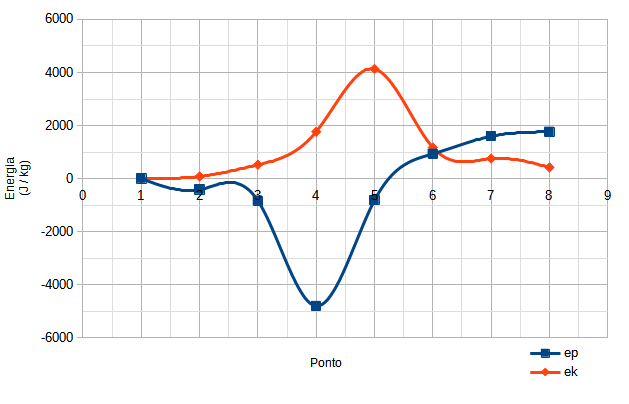
\includegraphics[scale = 0.60]{vent1.png}
\end{figure}

\begin{figure}[H]
    \caption{vazão 2}
    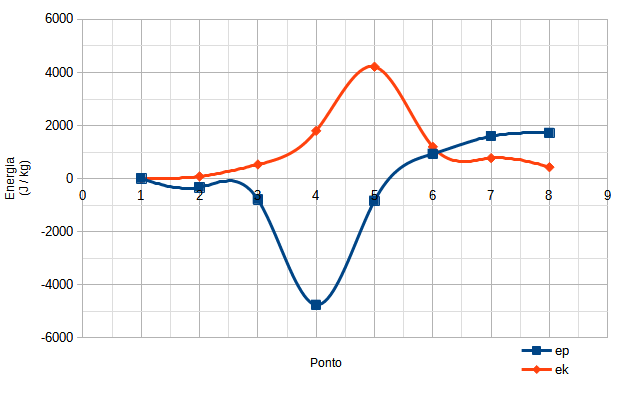
\includegraphics[scale = 0.60]{vent2.png}
\end{figure}



\section{Conclusão}

\tab Infelizmente podemos notar que a partir do ponto 5 a energia potencial não segue exatamente
o esperado, e acaba por assumir valores positivos, também é perceptível um atraso entre a relação das curvas.
E por fim um espaçamento entre as curvas.

Pode se a atribuir os valores positivos da energia potencial que seu valor padrão no ponto 1 é relacionado a uma
pressão negativa e assim quando a pressão se tornou positiva, em relação a pressão atmosférica, a energia potencial
se apresentou como positiva então, não havendo uma criação de energia no sistema. O \emph{delay} pode ter ocorrido
devido a natureza dos calculos empregados de variação de energia. e a abertura entre as curvas se deve a energias 
residuais como a de fricção, de natureza entrópica.


\end{document}
